\documentclass[12pt,a4paper]{article}
\usepackage[utf8]{inputenc}
\usepackage[T2A]{fontenc}
\usepackage[russian]{babel}
\usepackage{graphicx}
\usepackage{booktabs}
\usepackage{longtable}
\usepackage{geometry}

\usepackage{float}

\geometry{top=2cm, left=2cm, right=2cm, bottom=2cm}
\usepackage{paracol}
\usepackage{src/title}
\usepackage{hyperref}

\usepackage{listings}
\usepackage{xcolor}
\usepackage{listingsutf8}

\definecolor{codegreen}{rgb}{0,0.6,0}
\definecolor{codegray}{rgb}{0.5,0.5,0.5}
\definecolor{codepurple}{rgb}{0.58,0,0.82}
\definecolor{backcolour}{rgb}{0.95,0.95,0.92}

\lstdefinestyle{prolog}{
    inputencoding=utf8,
    extendedchars=true,
    backgroundcolor=\color{backcolour},
    commentstyle=\color{codegreen},
    keywordstyle=\color{magenta},
    numberstyle=\tiny\color{codegray},
    stringstyle=\color{codepurple},
    basicstyle=\ttfamily\footnotesize,
    breaklines=true,
    showstringspaces=false,
    numbers=left,
    numbersep=5pt,
    tabsize=2,
    captionpos=b,
    frame=single
}

\title{Лабораторная работа №1:\\База знаний Prolog и онтология в Protege (танки)}
\author{Ануфриев А.С. 465029}
\supervisor{Болдырева Е.А.}
\date{10.10.2026}

\abstract{
В рамках лабораторной работы выполнены два задания: (1) создана база знаний на Prolog по теме танков VII--VIII уровня, включающая 20+ фактов с одним аргументом, 15 фактов с двумя и более аргументами и 5 правил; написаны запросы разной сложности с использованием переменных, логических операторов (И, ИЛИ, НЕ) и правил; (2) переведена база знаний в онтологическую форму в Protege, описаны классы, свойства данных и объектные свойства, выполнена визуализация графа онтологии. Отчёт содержит описание выполненных шагов, примеры запросов и скриншоты с подписями.
}
\keywords{Prolog, онтология, Protege, OWL, база знаний, танки, логическое программирование}

\begin{document}
\maketitle

\section{Цели и задачи}

Цель работы --- развитие навыков работы с фактами, предикатами и правилами в логическом программировании (Prolog), а также знакомство с онтологическим моделированием в среде Protege и перевод базы знаний в форму OWL-онтологии.

Задачи:
\begin{enumerate}
    \item Создать базу знаний в Prolog (не менее 20 фактов с одним аргументом, 10--15 фактов с несколькими аргументами, 5--7 правил).
    \item Написать запросы разной сложности (простые, с переменными, с логическими операторами, с выполнением правил).
    \item Перевести базу знаний из Prolog в онтологию Protege (классы, свойства, экземпляры).
    \item Выполнить визуализацию онтологии и проверить её функциональность.
\end{enumerate}

\section{Теоретические сведения}

\subsection{Prolog}
Prolog --- язык логического программирования, основанный на логике предикатов первого порядка. Программа состоит из фактов, правил и запросов. Факты описывают отношения; правила позволяют выводить новые факты на основе существующих.

\subsection{Онтология}
Онтология --- формальное описание предметной области в виде классов, свойств и экземпляров. Формат OWL используется в Protege для создания и редактирования онтологий. Рассуждатель (reasoner) позволяет проверять согласованность и выводить новые знания из аксиом.

\section{Ход работы}

\subsection{Часть 1. База знаний в Prolog}

Создана база знаний на тему танков VII--VIII уровня. Файл \texttt{lab\_1/prog/tanks.pl} содержит:

\textbf{Факты с одним аргументом (20+):} нации (ussr, germany, usa), классы техники (heavy, medium, tank\_destroyer), производители, уровни (7, 8) и список танков (is\_3, t\_44, tiger\_i и др.).

\textbf{Факты с двумя и более аргументами (15):} \texttt{tank\_stats/11} (уровень, нация, класс, HP, урон, пробитие, броня, калибр, название, перезарядка); \texttt{built\_by/3} (танк, производитель, год); \texttt{unlocked\_from/2} (танк VIII $\leftarrow$ танк VII); \texttt{team/2} и \texttt{team\_title/2}.

\textbf{Правила (5):}
\begin{itemize}
    \item \texttt{durable(T)} --- танк с HP $\geq 1800$;
    \item \texttt{hard\_hitter(T)} --- пробитие $\geq 220$ мм;
    \item \texttt{all\_rounder(T)} --- конъюнкция \texttt{durable} и \texttt{hard\_hitter};
    \item \texttt{glass\_cannon(T)} --- \texttt{hard\_hitter} И НЕ \texttt{durable};
    \item \texttt{opponents(A,B)} --- пары противников (Германия против СССР/США) с использованием дизъюнкции (;);
    \item \texttt{best\_gun(Lvl, T)} --- лучший танк по пробитию на уровне Lvl.
\end{itemize}

\textbf{Примеры запросов (из \texttt{tanks.pl}, раздел 4):}

Ниже приведены запросы в формате \texttt{ввод $\rightarrow$ вывод}.

\textbf{4.1 Простые запросы:}

\begin{lstlisting}[style=prolog,language={},numbers=none,frame=none,basicstyle=\ttfamily\small]
?- tank(is_3).
true
?- tank(is_1).
false
?- nation(germany).
true
?- level(7).
true
?- manufacturer(henschel).
true
?- tank_class(heavy).
true
?- built_by(is_3, M, Y).
M = chelyabinsk_kirov_plant, Y = 1945
?- unlocked_from(t_44, P).
P = t_43
?- team(ussr_8, L).
L = [is_3, t_44, isu_152]
?- team_title(usa_7, T).
T = '7 уровень США'
\end{lstlisting}

\textbf{4.2 Запросы с переменными:}

\begin{lstlisting}[style=prolog,language={},numbers=none,frame=none,basicstyle=\ttfamily\small]
?- tank_stats(T, 8, ussr, _, _, _, _, _, _, _, _).
T = is_3 ; T = t_44 ; T = isu_152

?- tank_stats(T, _, _, heavy, HP, _, _, _, _, _, _), HP > 1800.
T = tiger_ii ; T = t32

?- tank_stats(T, _, _, _, _, Alpha, _, _, _, _, _), Alpha >= 400.
T = is_3 ; T = t_44 ; T = isu_152 ; T = jpanther ; T = ferdinand ;
T = t_29 ; T = t_28_prot ; T = su_152

?- tank_stats(T, 7, usa, _, _, _, _, _, Name, _, _).
T = t29, Name = 'T29' ; T = t_20, Name = 'T20' ; T = t_25_2, Name = 'T25/2'

?- tank_stats(T, _, _, _, _, _, Pen, _, _, _, Reload), Pen >= 220, Reload =< 12.
T = is_3 ; T = isu_152 ; T = tiger_ii ; T = ferdinand ; T = t28_prot
\end{lstlisting}

\textbf{4.3 Логические операторы (И / ИЛИ / НЕ):}

\begin{lstlisting}[style=prolog,language={},numbers=none,frame=none,basicstyle=\ttfamily\small]
% И: уровень 8, СССР, HP > 1500
?- tank_stats(T, 8, ussr, _, _, _, _, _, _, _, _),
   tank_stats(T, _, _, _, HP, _, _, _, _, _, _), HP > 1500.
T = is_3

% ИЛИ: средний или ПТ-САУ
?- tank_stats(T, _, _, medium, _, _, _, _, _, _, _) ;
   tank_stats(T, _, _, tank_destroyer, _, _, _, _, _, _, _).
T = t_44 ; T = panther_i ; T = panther_ii ; T = t_20 ; T = pershing ;
T = isu_152 ; T = jpanther ; T = ferdinand ; T = t_25_2 ; T = t28_prot ; T = su_152

% НЕ: не живучие танки
?- tank(T), \+ durable(T).
T = t_44 ; T = isu_152 ; T = tiger_i ; T = panther_i ; T = jpanther ;
T = panther_ii ; T = ferdinand ; T = t29 ; T = t_20 ; T = t_25_2 ;
T = pershing ; T = t28_prot ; T = is ; T = t_43 ; T = su_152
\end{lstlisting}

\textbf{4.4 Запросы с выполнением правил:}

\begin{lstlisting}[style=prolog,language={},numbers=none,frame=none,basicstyle=\ttfamily\small]
?- durable(T).
T = is_3 ; T = tiger_ii ; T = t32

?- hard_hitter(T).
T = is_3 ; T = isu_152 ; T = jpanther ; T = tiger_ii ;
T = ferdinand ; T = t28_prot ; T = su_152

?- all_rounder(T).
T = is_3 ; T = tiger_ii

?- glass_cannon(T).
T = isu_152 ; T = jpanther ; T = ferdinand ; T = t28_prot ; T = su_152

?- opponents(A, B).
A = tiger_i, B = is ; A = is_3, B = tiger_ii ; ...

?- best_gun(8, T).
T = isu_152 (пробитие 286)

?- best_gun(7, T).
T = su_152 (пробитие 250)
\end{lstlisting}

\subsection{Часть 2. Онтология в Protege}

Онтология переведена из Prolog в OWL. Файл \texttt{lab\_1/prog/tanks\_ontology.ttl} содержит:

\textbf{Классы:} Tank и подклассы HeavyTank, MediumTank, TankDestroyer (дизъюнктные); Nation; Manufacturer; Level; Team; а также определённые классы: DurableTank, HardHitter, AllRounder, GlassCannon, SovietTank, GermanTank, AmericanTank, AlliedTank, Tier7Tank, Tier8Tank.

\textbf{Объектные свойства:} hasNation, hasLevel, builtBy (и inverse produced), unlockedFrom (и inverse leadsTo), hasMember, sameManufacturerAs (цепочка свойств).

\textbf{Свойства данных:} hasName, hasHP, hasAlphaDamage, hasPenetration, hasFrontArmor, hasCaliber, hasReloadTime, developmentStartYear, levelNumber, teamTitle.

\textbf{Экземпляры:} все 18 танков с характеристиками, производители, команды (Team\_USSR\_8, Team\_Germany\_8 и др.).

Визуализация графа онтологии сохранена как \texttt{lab\_1/images/graph.png} и сгенерирована из \texttt{lab\_1/prog/ontoGraf.graph}.

\subsection{Скриншоты выполнения (Protege)}

Ниже приведены скриншоты из среды Protege и визуализации онтологии.

\begin{center}
    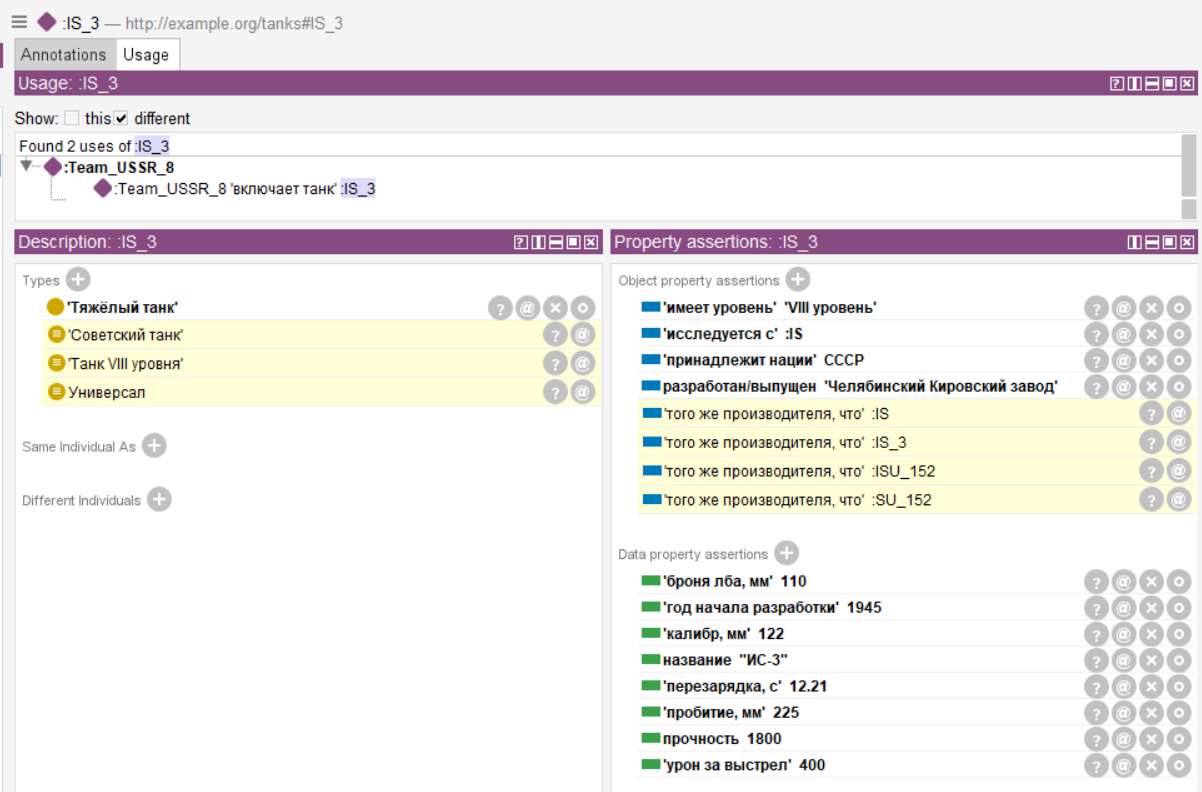
\includegraphics[width=0.85\textwidth]{../images/example_1.png}
\end{center}

\begin{center}
    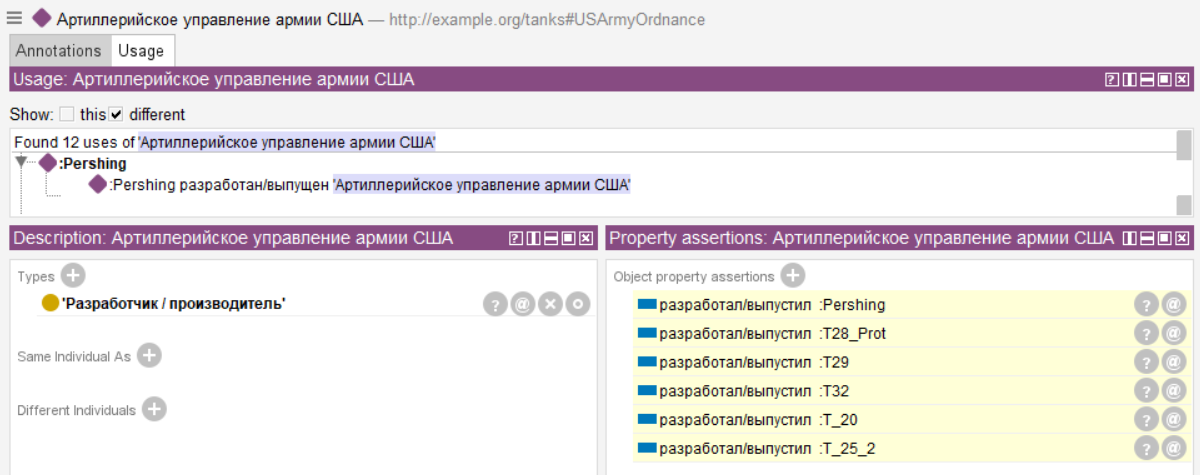
\includegraphics[width=0.85\textwidth]{../images/example_2.png}
\end{center}

\begin{center}
    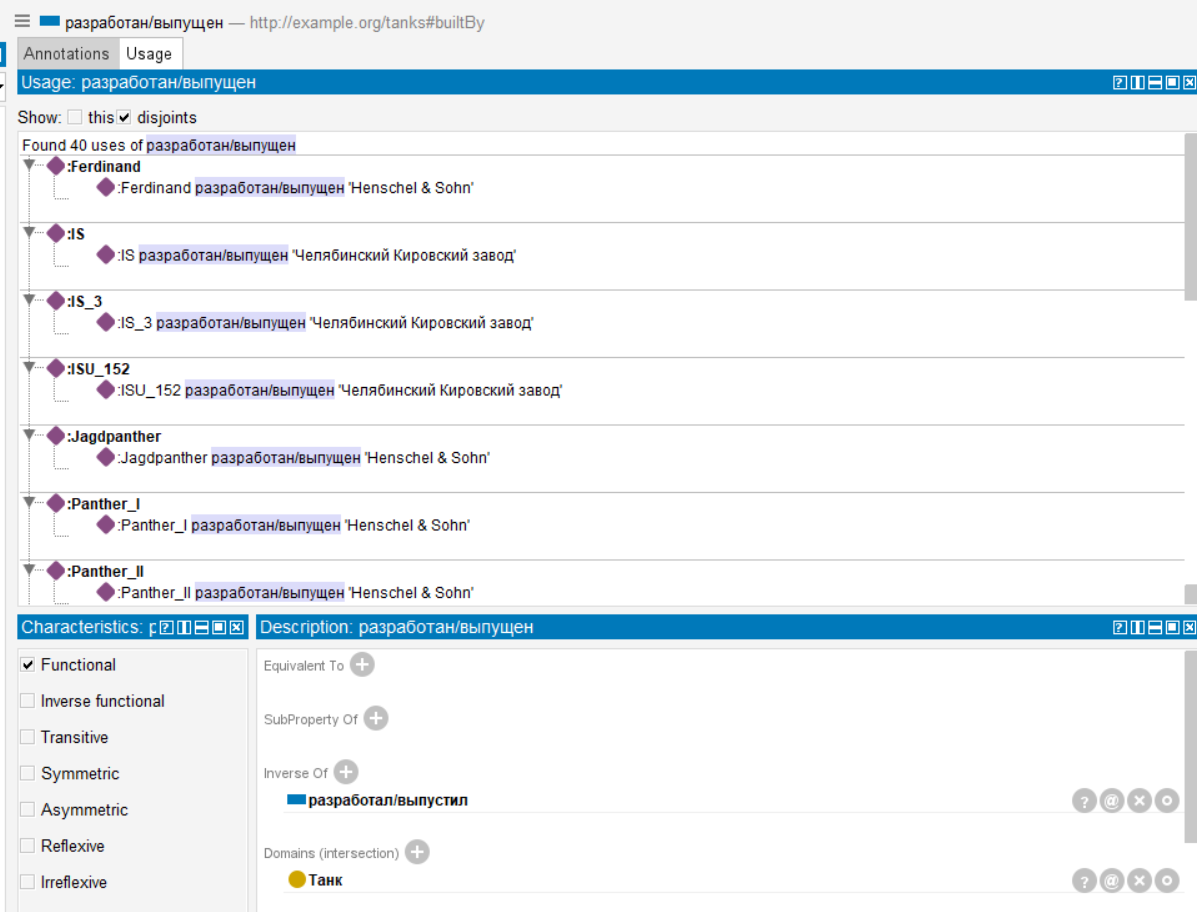
\includegraphics[width=0.85\textwidth]{../images/example_3.png}
\end{center}

\begin{center}
    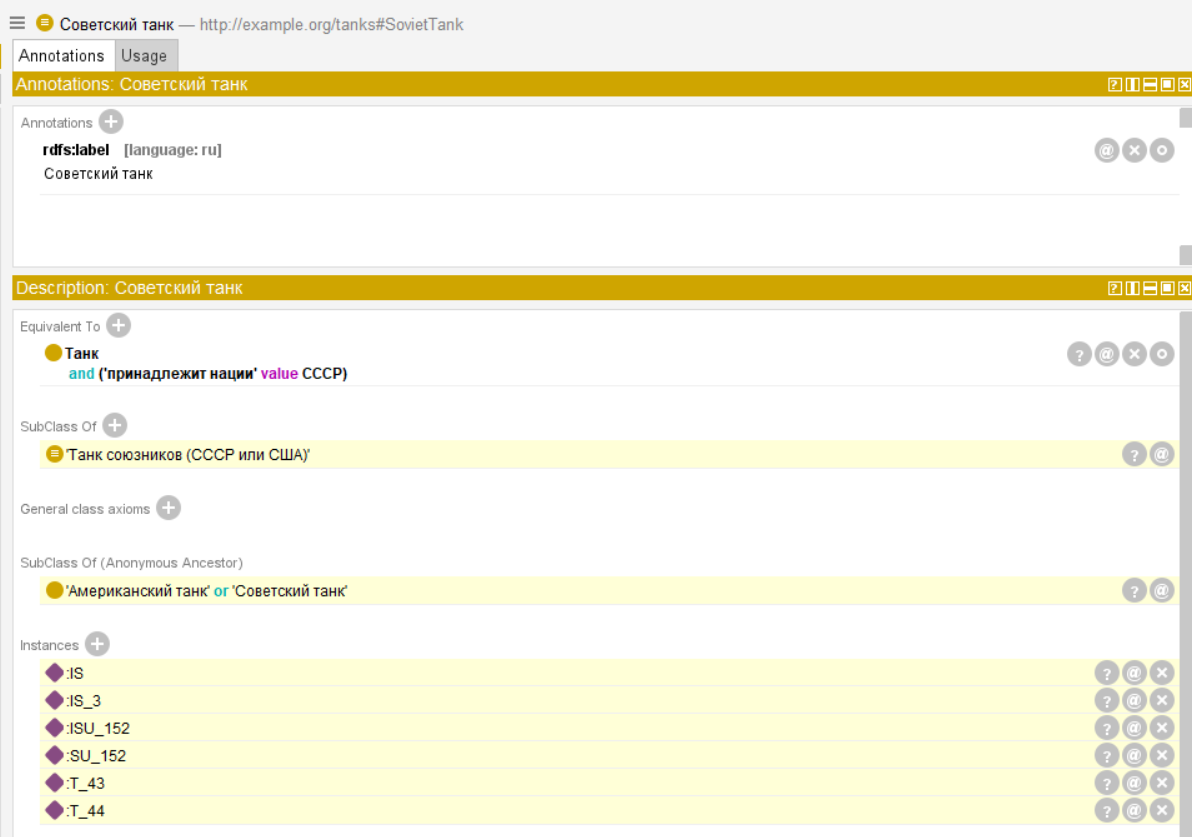
\includegraphics[width=0.85\textwidth]{../images/example_4.png}
\end{center}

\section{Результаты, код, графики, таблицы, анализ}

\subsection{Статистика базы знаний}

\begin{table}[H]
\centering
\caption{Количественные характеристики базы знаний}
\begin{tabular}{l|c}
\toprule
Компонент & Количество \\
\midrule
Факты с одним аргументом & 23 (нации, классы, производители, уровни, танки) \\
Факты с двумя аргументами & 15 (tank\_stats/11 включает несколько аргументов) \\
Правила & 6 (durable, hard\_hitter, all\_rounder, glass\_cannon, opponents, best\_gun) \\
Запросы (примеров в коде) & 20+ (простые, с переменными, с операторами, с правилами) \\
Танков в базе & 18 \\
Команд & 6 \\
\bottomrule
\end{tabular}
\end{table}

\subsection{График онтологии}

На рисунке \ref{fig:graph} представлен визуализированный граф онтологии (из файла \texttt{graph.png}). Видны классы (Tank, HeavyTank, MediumTank, TankDestroyer, Nation, Manufacturer, Team и др.) и связи между экземплярами.

\begin{figure}[H]
    \centering
    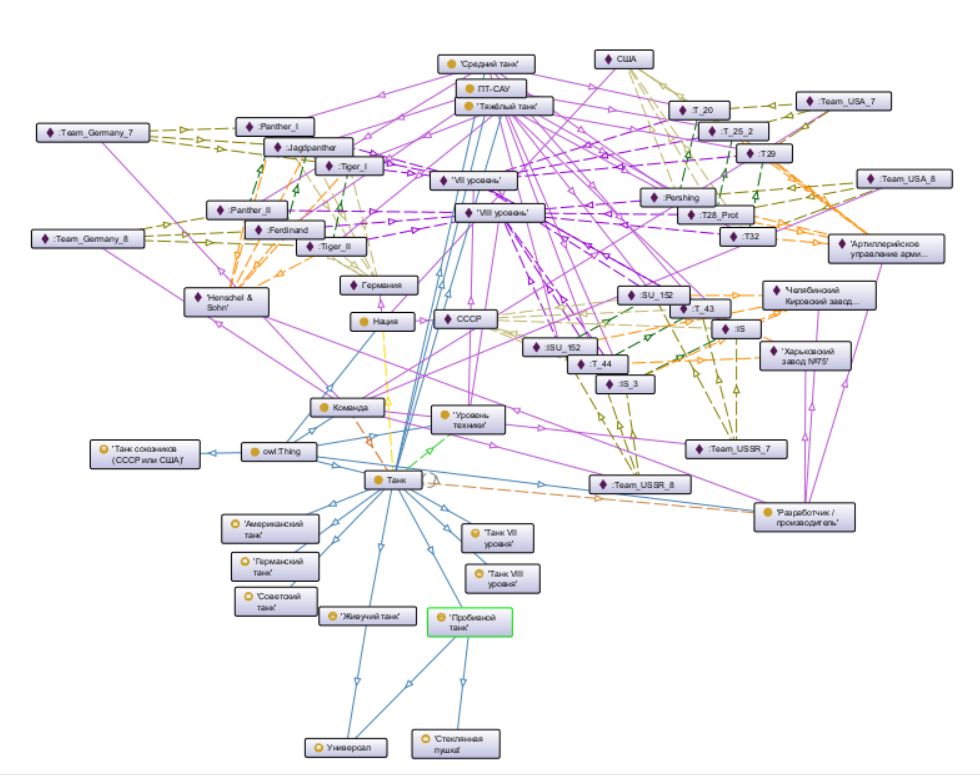
\includegraphics[width=0.85\textwidth]{../images/graph.png}
    \caption{Граф онтологии танков (Protege / OntoGraf).}
    \label{fig:graph}
\end{figure}

\subsection{Анализ запросов}

Простые запросы возвращают конкретные факты. Запросы с переменными позволяют искать по условиям (например, все тяжёлые танки с HP $> 1800$). Логические операторы обеспечивают сложные фильтры. Правила \texttt{durable} и \texttt{hard\_hitter} формализуют критерии; \texttt{all\_rounder} и \texttt{glass\_cannon} демонстрируют конъюнкцию и отрицание. Правило \texttt{opponents} показывает работу с дизъюнкцией. \texttt{best\_gun} использует агрегацию.

В онтологии эквиваленты правил выражены через \texttt{owl:equivalentClass} с \texttt{owl:intersectionOf} и \texttt{owl:complementOf}, что позволяет рассуждателю (HermiT) автоматически классифицировать экземпляры в классы DurableTank, HardHitter, AllRounder, GlassCannon и др.

\section{Выводы}

В ходе работы успешно выполнены оба задания лабораторной работы №1:
\begin{itemize}
    \item Создана полноценная база знаний Prolog по теме танков с достаточным количеством фактов и правил; написаны запросы разной сложности, демонстрирующие использование переменных и логических операторов.
    \item База знаний переведена в онтологию OWL в Protege; определены классы, свойства и экземпляры; выполнена визуализация графа онтологии.
    \item Проверена функциональность онтологии (через аксиомы классов и возможности рассуждателя).
\end{itemize}

Работа показала взаимосвязь между логическим программированием и онтологическим моделированием: факты и правила Prolog естественным образом отображаются в экземпляры, классы и аксиомы OWL.

\section{Приложение. Код базы знаний Prolog}

Полный текст файла \texttt{../prog/tanks.pl} приведён ниже с нумерацией строк и подсветкой синтаксиса.

\lstinputlisting[style=prolog,language={},caption={Файл tanks.pl},label={lst:tanks},inputencoding=utf8,extendedchars=true]{../prog/tanks.pl}


\end{document}
